\section{Algorithm}\label{sec:solution}

\ag{Explain the quality function and why it is a good proxy for the optimization function that you presented in \Cref{sec:model}, add proposition and proof for its sensitivity, add the algorithms (use the one-shot-top-k mechanism which is equivalent to k times the exponential mechanism, see~\cite{TaoGMR22}), write the pseudo code, add a textual explanation for the code, and a proposition and proof for the algorithm being DP.}

\ag{Challenges: (1) generating all possible views is impossible so considering only views that are expressed by predicates (common in explanation works), (2) the optimization function has high sensitivity and high computational cost even with views generated by predicates so we define a proxy function with limited sensitivity that can be easily computed.}


Designing a practical algorithm for private query-refinement explanations requires addressing two central challenges: the enormous combinatorial space of potential views and the high sensitivity of the optimization objective defined in Section~3. Directly optimizing this objective is computationally infeasible and would yield poor differential privacy guarantees. To overcome these obstacles, our approach introduces a carefully crafted proxy quality function with bounded sensitivity, enabling efficient evaluation under differential privacy. We then propose the following framework for the solution of this problem as shown in figure \ref{fig:query-refinement}:

\begin{figure}[ht]
\centering
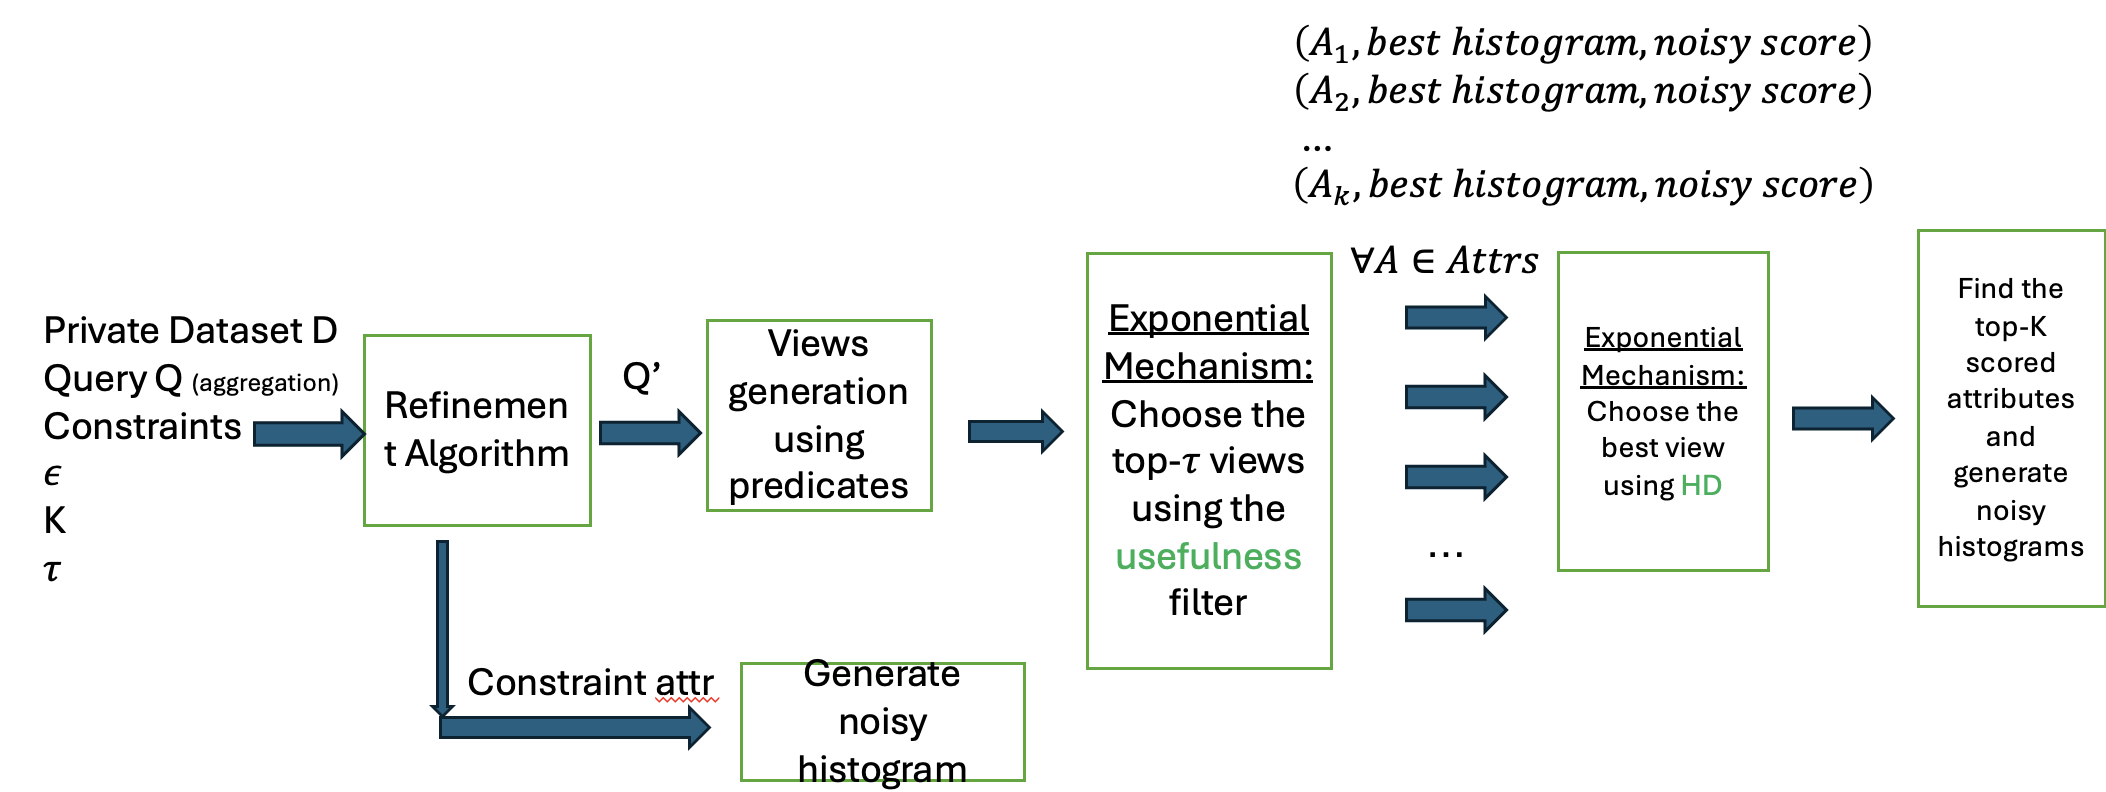
\includegraphics[width=0.8\linewidth]{figures/new private query refinement framework.png}
\caption{An illustration of the framework}
\label{fig:query-refinement}
\end{figure}

\begin{enumerate}
    \item Given a private database $D$, a query $Q$, and a constraints set $\mathcal{C}$, we run a refinement mechanism and get a refinement $Q'$ that satisfies the constraints.
    \item Generate a set of predicate views of the data that will form the basis on top of which we will create the histograms.
    \item Filter out views that are "less useful" in terms of explaining trends. According to a usefulness measure which is a proxy function with low sensitivity (e.g. views that are very small, or that are very different from the original database in the distribution of the features). 
    \item For each attribute, find the view that best reflects the change between the results of $Q(D)$ and $Q'(D)$ for this attribute, in terms of the difference in the one-way marginals of this attribute.
    \item Release the best-$k$ noisy histograms of the different attributes from the set of tuples (Attribute, Best View, Noisy Score) we collected in the previous step.
\end{enumerate}

\subsection{Proxy Measures}
We introduce the proxy functions for the Usefulness and the one-way marginals (Histograms Distance) and proof they are sensitive bounded.

% \begin{algorithm}[H]
% \caption{Views-Gen}
% \label{alg:views-gen}
% \begin{algorithmic}[1]
% \REQUIRE 
% \begin{itemize}
%   \item Attributes: Set of available attributes
%   \item D: Private dataset
% \end{itemize}

% \STATE $\mathcal{P} \leftarrow \emptyset$

% \FOR{each $A_i,A_j \in Attributes \times Attributes$}
%     \FOR{each $V_i, V_j \in Dom(D[A_i])\times Dom(D[A_j])$}
%         \STATE $P \leftarrow \{t\in D | t[A_i]=V_i, t[A_j]=V_j\}$
%         \STATE $\mathcal{P} \leftarrow \mathcal{P} \cup \{P\}$
%     \ENDFOR
% \ENDFOR

% \RETURN $\mathcal{P}$.
% \end{algorithmic}
% \end{algorithm}

\begin{definition}[Histogram Distance]  
Given a dataset $D$, a view predicate $p$, an attribute $A$, 
and two queries $Q$ and $Q'$,  
the \emph{Histogram Distance} (HD) is defined as:
\begin{align}
HD &= \sum_{V \in \text{buckets}(D[A])} 
\frac{\left| H_{Q(p(D)),A}(V) - H_{Q'(p(D)),A}(V) \right|}
     {H_{p(D),A}(V)},
\label{eq:hd-definition}
\end{align}
where $H_{Q(p(D)),A}(V)$ denotes the count of records in bucket $V$ for attribute $A$
in the result of $Q$ applied to $p(D)$,  
and $H_{p(D),A}(V)$ is the total count in bucket $V$ for $p(D)$.
\end{definition}

\begin{proposition}
The global sensitivity of $HD$ as defined in~\eqref{eq:hd-definition} is at most $1$, and its range is $0 \le \mathrm{HD}(D) \le |p(D)|$.
\end{proposition}

\begin{proof}
Let $D, D'$ be neighboring datasets such that $|\,|D'| - |D|\,| = 1$ and $D' = D \cup \{t\}$,  
where $t$ is a single tuple.  
Let $t_A = V'$ denote the bucket value for attribute $A$ of tuple $t$.

The global sensitivity of $HD$ is:
\begin{equation}
GS_{HD} = \max_{\substack{D,D' \\ D \sim D'}} 
\left| HD(D) - HD(D') \right|,
\end{equation}
where $D \sim D'$ denotes that $D$ and $D'$ are neighboring datasets.

From~\eqref{eq:hd-definition}, we have:
\begin{align}
&\left| HD(D) - HD(D') \right| \notag \\
&= \bigg| 
\sum_{V \in \text{buckets}(D'[A])} 
\frac{\left| H_{Q(p(D)),A}(V) - H_{Q'(p(D)),A}(V) \right|}
     {H_{p(D),A}(V)} \notag \\
&\quad - 
\sum_{V \in \text{buckets}(D'[A])} 
\frac{\left| H_{Q(p(D')),A}(V) - H_{Q'(p(D')),A}(V) \right|}
     {H_{p(D'),A}(V)}
\bigg|.
\end{align}

We partition the set of buckets into two disjoint subsets:
\[
\text{buckets}(D'[A]) = 
\left(\text{buckets}(D'[A]) \setminus \{V'\}\right) \cup \{V'\}.
\]

\textbf{Case 1: $V \neq V'$}.  
For all $V \neq V'$, the numerator in each term is unchanged between $D$ and $D'$,  
while the denominator changes by at most $1$ because the tuple $t$ is not assigned to $V$.  
Thus:
\[
\sum_{V\ne V' \in \text{buckets}(D'[A])} \left| 
\frac{\cdot}{H_{p(D),A}(V)} - \frac{\cdot}{H_{p(D'),A}(V)}
\right| \leq 1.
\]

\textbf{Case 2: $V = V'$}.  
Here, both numerator and denominator may change, but by the neighboring dataset property,  
each changes by at most $1$. Therefore:
\begin{align}
&\left| 
\frac{\left| H_{Q(p(D)),A}(V') - H_{Q'(p(D)),A}(V') \right|}{H_{p(D),A}(V')}
\right. \notag \\
&\quad \left.
-
\frac{\left| H_{Q(p(D')),A}(V') - H_{Q'(p(D')),A}(V') \right|}{H_{p(D'),A}(V')}
\right| \leq 1.
\end{align}



Since only one bucket $V'$ can change between $D$ and $D'$,  
and the change in that bucket’s contribution is bounded by $1$,  
it follows that:
\[
\left| HD(D) - HD(D') \right| \leq 1.
\]

Taking the maximum over all neighboring datasets yields:
\[
GS_{HD} \leq 1.
\]
\end{proof}

\begin{definition}[Similarity Penalty]
Let $D$ be a dataset, $\mathcal{A}$ a set of attributes and $A^*$ an attribute.
We define the Similarity Penalty of $A^*$ with respect to $D, \mathcal{A}$ as following:
\begin{equation}
SimilarityPenalty(A^*,\mathcal{A}, D) \;=\; TVD(D[A^*], D[\mathcal{A}])
\end{equation}
\end{definition}

\begin{definition}[Usefulness Index]
Let $D$ be a dataset, $p$ a view predicate, $A$ an attribute, and $Q_1,Q_2$ two queries.
We define the coverage index as following:
\begin{equation}
Coverage(p,Q_1, Q_2, D) \;=\; \frac{|Q_1(p(D))| + |Q_2(p(D))|}{|D|}
\end{equation}
Let $Representativeness(p, D) := \mathrm{TVD}(D, p(D))$ denote the total variation distance as a Representativeness index.  
The \emph{Usefulness index} is defined as
\begin{equation}
Usefulness(p,Q_1,Q_2,D) = Representativeness(p,D) \cdot Coverage(p,Q_1,Q_2,D)
\end{equation}
\end{definition}

\begin{proposition}[Global sensitivity of $Usefulness$]
Using previous works that showed: \alon{Add reference}
\begin{enumerate}
  \item $\mathrm{TVD}(\cdot) \in [0,1]$
  \item $\mathrm{GS}_{\mathrm{TVD}} = 1/|D|$ ,
\end{enumerate}
Then
\[
\mathrm{\Delta}_{Usefulness} \;=\; \max_{D\sim D'} |U(D) - U(D')| \; \leq \; 4.
\]
and its range is bounded by $0 \le Usefulness(D) \le \frac{2|p(D)|^2}{|D|}$.
\end{proposition}

\begin{proof}
Let $D, D'$ be neighboring datasets with $D' = D \cup \{t\}$.
We denote:
\[
x = \mathrm{TVD}(p,D), \quad
y = Coverage(p,Q,Q',D),
\]
and similarly 
\[
x' = \mathrm{TVD}(p,D'), \quad
y' = Coverage(p,Q,Q',D')
\].

Therefore, we have:
\begin{align}
&|Usefulness(p,Q,Q',D) - Usefulness(p,Q,Q',D')| \;=\; |x y - x' y'| 
\notag \\
&= |xy - x'y + x'y - x'y'|
   \leq |x - x'|\,|y|
   + |y - y'|\,|x'| \label{eq:useful-diff-ineq}
\end{align}

\paragraph{(i) First term bound.}
We can bound \(|y| \leq 2\):
\[
y \;=\; \frac{|Q(p(D))| + |Q'(p(D))|}{|D|} \; \leq \; \frac{|D| + |D|}{|D|} \;=\; 2,
\]
Therefore, we get:
\begin{equation}
|x - x'|\,|y|\;\leq\; |x - x'| \cdot 2
\;\leq\; 2 \cdot \mathrm{GS}_{\mathrm{TVD}} = 2/|D|.
\label{eq:term1-bound}
\end{equation}

\paragraph{(ii) Second term bound.}
\begin{align}
&|y - y'| \;=\;
\left| \frac{|Q(p(D))| + |Q'(p(D))|}{|D|}
     - \frac{|Q(p(D'))| + |Q'(p(D'))|}{|D'|} \right| \notag \\
&= \left| \frac{|Q(p(D))| + |Q'(p(D))|}{|D|}
     - \frac{|Q(p(D'))| + |Q'(p(D'))|}{|D|+1} \right| \notag \\
&\leq \left| \frac{|Q(p(D'))|}{|D|+1} - \frac{|Q(p(D))|}{|D|} \right| + \left| \frac{|Q'(p(D'))|}{|D|+1} - \frac{|Q'(p(D))|}{|D|} \right| \notag \\
&= \left| \frac{|Q(p(D'))|\cdot |D|- |Q(p(D))| \cdot (|D|+1)}{|D|(|D|+1)} \right| + \notag\\
&\left| \frac{|Q'(p(D'))|\cdot |D| - |Q'(p(D))|\cdot (|D|+1)}{|D|(|D|+1)} \right| \notag \\
&= \left| \frac{|D|\cdot (|Q(p(D'))|- |Q(p(D))|) -|Q(p(D))|}{|D|(|D|+1)} \right| + \notag\\
&\left| \frac{|D|\cdot (|Q'(p(D'))| - |Q'(p(D))|) - |Q'(p(D))|}{|D|(|D|+1)} \right| \notag \\
&= \left| \frac{|Q(p(D'))|- |Q(p(D)))}{|D| + 1} - \frac{|Q(p(D))|}{|D|(|D|+1)} \right| + \notag\\
&\left| \frac{|Q'(p(D'))| - |Q'(p(D))|}{|D| + 1} - \frac{|Q'(p(D))|}{|D|(|D|+1)} \right| \notag \\
&\leq \left| \frac{1}{|D| + 1} + \frac{|Q(p(D))|}{|D|(|D|+1)} \right| + \left| \frac{1}{|D| + 1} + \frac{|Q'(p(D))|}{|D|(|D|+1)} \right| \notag \\
&\leq 1+1 =2.
\end{align}

Therefore:
\begin{equation}
|y - y'|\,|x'|\;\leq\; 2\cdot 1=2.
\label{eq:term2-bound}
\end{equation}

\paragraph{(iii) Combine.}
From \eqref{eq:useful-diff-ineq}, \eqref{eq:term1-bound} and \eqref{eq:term2-bound}:
\begin{align}
|Usefulness(p,Q,Q',D) - Usefulness(p,Q,Q',D')| &\leq 2 +2 = 4.
\end{align}
Therefore, \(\mathrm{GS}_{Usefulness} \leq 4\).
\end{proof}

\subsection{Solving the Private Query-Refinement Explanations Problem}
in this subsection we introduce our algorithm for solving the Private Query-Refinement Explanations problem.
We first introduce the overall algorithm which implements the framework of figure \ref{fig:query-refinement} and then the auxiliary algorithms it uses. Then we show that each algorithm is $\epsilon-DP$ and conclude that the overall algorithm is also $\epsilon-DP$.
% \begin{algorithm}[H]
% \caption{Private-Query-Refinement-Explanation}
% \label{alg:private-query-refinement}
% \begin{algorithmic}[1]
% \REQUIRE 
% \begin{itemize}
%   \item $D$: A private dataset.
%   \item Attributes: Set of available attributes
%   \item $Q$: SPJ Query
%   \item $RM$: Refinement mechanism
%   \item $\mathcal{C}$: Set of cardinality-constraints
%   \item $\tau$
%   \item $k$
%   \item $\epsilon$: Privacy budget 
% \end{itemize}

% \STATE $Q' \leftarrow RM(Q, D, \mathcal{C})$
% \STATE //Views Genetation
% \STATE $\mathcal{P} \leftarrow \emptyset$


% \FOR{each $A_i,A_j \in Attributes \times Attributes$}
%     \FOR{each $V_i, V_j \in Dom(D[A_i])\times Dom(D[A_j])$}
%         \STATE $P \leftarrow \{t\in D | t[A_i]=V_i, t[A_j]=V_j\}$
%         \STATE $\mathcal{P} \leftarrow \mathcal{P} \cup \{P\}$
%     \ENDFOR
% \ENDFOR
% \STATE $\hat{\mathcal{P}} \leftarrow \text{One-Shot Top-}\tau(\mathcal{P}, D, Usefullness, \frac{\epsilon}{3})$
% \STATE $Cands\leftarrow Candidates-Gen(Attributes, \hat{\mathcal{P}}, Q, Q', \frac{\epsilon}{3})$
% \RETURN $\text{Find-Top-k-Explanations}(Attributes, Cands, Q, Q', k, \frac{\epsilon}{3})$
% \end{algorithmic}
% \end{algorithm}

\begin{algorithm}[t]
\caption{Private-Queries-Diff-Top-$k$-Explanation}
\label{alg:main}
\begin{algorithmic}[1]
\Require Private dataset $D$; queries $Q_1, Q_2$; predicate-based views $\mathcal{P}$; attribute set $\textit{Attrs}$; threshold $\tau$; number of explanations $k$; privacy budget $\epsilon$
\Ensure A set of $k$ differentially private explanation histograms

\Statex \textbf{Overview.} Privately select a subset of informative views, generate candidates, and privately select and release the top-$k$ explanations.
\State \textbf{/* Privacy budget allocation */}
\State $\epsilon_P, \epsilon_S, \epsilon_H  \gets \epsilon/2, \epsilon/4, \epsilon/4$


\State \textbf{/* Private view selection */}
\State Define $u_{\text{use}}(p) \gets \textit{Usefulness}(p, D, Q_1, Q_2)$
\State $\hat{\mathcal{P}}  \gets \textsc{OneShotTop-}\tau(\mathcal{P}, u_{\text{use}}(\cdot), \epsilon_P)$
\Comment{$\epsilon_P$-DP}

\Statex \textbf{(Post-processing)} Candidate construction does not incur additional privacy loss.

\State \textbf{/* Construct explanation candidates */}
\State $C \gets \emptyset$
\ForAll{$p \in \hat{\mathcal{P}}$}
    \ForAll{$A \in \textit{Attrs}$}
        \State $C \gets C \cup \{(p, A)\}$
    \EndFor
\EndFor

\State \textbf{/* Private top-$k$ explanation selection and release */}
\State $\mathcal{E} \gets \textsc{Find-Top-$k$-Explanations}(D, Q_1, Q_2, C, k, \epsilon_S, \epsilon_H)$

\Return $\mathcal{E}$
\end{algorithmic}
\end{algorithm}

\paragraph{Explanation of Algorithm~\ref{alg:main}.}
Algorithm~\ref{alg:main} orchestrates the end-to-end pipeline for generating differentially private explanations of query differences.

The algorithm begins by privately selecting a subset of informative predicate-based views using a One-Shot Top-$\tau$ mechanism. This mechanism uses the \emph{Usefulness} score, defined earlier in the paper, as its utility function. Since the sensitivity of the Usefulness score is bounded, the view selection step satisfies $\epsilon_P$-differential privacy. The construction of explanation candidates by pairing selected views with attributes is purely deterministic and therefore constitutes post-processing, incurring no additional privacy loss. Finally, the algorithm invokes Algorithm~\ref{alg:topk} to privately select and release the top-$k$ explanations. By design, Algorithm~\ref{alg:main} does not directly release any data-dependent statistics. all privacy-sensitive operations are delegated to differentially private subroutines whose composition yields the final privacy guarantee.


\begin{algorithm}[t]
\caption{Find-Top-$k$-Explanations}
\label{alg:topk}
\begin{algorithmic}[1]
\Require Private dataset $D$; queries $Q_1,Q_2$; candidates $C$; $k$; budgets $\epsilon_S,\epsilon_H$
\Ensure $k$ differentially private explanation histograms

\State $ChosenAttrs \gets \emptyset$
\State $\mathcal{E} \gets \emptyset$

\For{$i \gets 1$ to $k$}

  \State \textbf{/* Private selection using EM */}
  \State $u_{i,chosenAttrs}(c=(p,A)) := HD(D; p,A,Q_1,Q_2) \cdot DiversityScore(A,ChosenAttrs)$
  \State $c_i=(p_i,A_i) \gets \textsc{ExponentialMechanism}( \newline C, u_{i, ChosenAttrs}(\cdot), \epsilon_S/k)$

  \State \textbf{/* Private histogram release */}
  \State $\Delta H_i(V) \gets H_{Q_1(p_i(D)),A_i}(V)-H_{Q_2(p_i(D)),A_i}(V)$
  \State $\widetilde{\Delta H_i} \gets \Delta H_i + \textsc{Laplace}(2k/\epsilon_H)$

  \State $\mathcal{E} \gets \mathcal{E} \cup \{\widetilde{\Delta H_i}\}$
  \State $ChosenAttrs \gets ChosenAttrs \cup \{A_i\}$
  \State $C \gets C \setminus \{c_i\}$

\EndFor


\State \Return $\mathcal{E}$
\end{algorithmic}
\end{algorithm}

\paragraph{Explanation of Algorithm~\ref{alg:topk}.}
Algorithm~\ref{alg:topk} is responsible for selecting and releasing the final explanations under differential privacy. Given a set of explanation candidates, the algorithm proceeds iteratively for $k$ rounds. In each iteration, it computes a utility value for every remaining candidate, where the utility is defined as the histogram distance between the results of the two queries, optionally scaled by a diversity-aware factor that depends only on previously selected attributes. The bounded sensitivity of this utility function allows the algorithm to apply the exponential mechanism with a per-iteration privacy budget of $\epsilon_S/k$.

After selecting a candidate, the algorithm releases a noisy histogram that captures the difference between the two query results for the chosen view and attribute. Noise is added using the Laplace mechanism, calibrated to the sensitivity of the released histogram and a per-iteration budget of $\epsilon_H/k$. The selected candidate is then removed from further consideration, and the corresponding attribute is recorded to encourage diversity in subsequent selections. By sequential composition over the $k$ iterations, the selection and release steps together satisfy $(\epsilon_S + \epsilon_H)$-differential privacy. Any additional computations, such as updating the candidate set or tracking selected attributes, are post-processing steps and do not affect the privacy guarantees.

\subsection{Differential Privacy Analysis}
\label{subsec:dp-proof}

We now prove that Algorithms~\ref{alg:main} and~\ref{alg:topk} satisfy $\epsilon$-differential privacy with respect to the input private dataset $D$.

\begin{proposition}[Differential Privacy of Algorithm~\ref{alg:main}]
\label{thm:alg1-dp}
Algorithm~\ref{alg:main} satisfies $\epsilon$-differential privacy.
\end{proposition}

\begin{proof}
Algorithm~\ref{alg:main} receives a total privacy budget $\epsilon$ and explicitly partitions it into three components:
$\epsilon_P$ for private view selection,
$\epsilon_S$ for private explanation selection,
and $\epsilon_H$ for private histogram release,
such that $\epsilon_P + \epsilon_S + \epsilon_H = \epsilon$.

The first privacy-sensitive step in Algorithm~\ref{alg:main} is the selection of predicate-based views using a One-Shot Top-$\tau$ mechanism. This mechanism uses the \emph{Usefulness} score as its utility function. Since the sensitivity of the Usefulness score is bounded, the One-Shot Top-$\tau$ mechanism satisfies $\epsilon_P$-differential privacy.

All subsequent operations prior to invoking Algorithm~\ref{alg:topk}, including the construction of explanation candidates by pairing selected views with attributes, are deterministic functions of the output of the private view selection step. By the post-processing property of differential privacy, these operations incur no additional privacy loss.

Algorithm~\ref{alg:main} then invokes Algorithm~\ref{alg:topk}, passing to it the remaining privacy budgets $\epsilon_S$ and $\epsilon_H$. As shown in Theorem~\ref{thm:alg2-dp}, Algorithm~\ref{alg:topk} satisfies $(\epsilon_S + \epsilon_H)$-differential privacy. By sequential composition of differentially private mechanisms, the overall privacy loss of Algorithm~\ref{alg:main} is bounded by
$\epsilon_P + \epsilon_S + \epsilon_H = \epsilon$.

Therefore, Algorithm~\ref{alg:main} satisfies $\epsilon$-differential privacy.
\end{proof}

\begin{proposition}[Differential Privacy of Algorithm~\ref{alg:topk}]
\label{thm:alg2-dp}
Algorithm~\ref{alg:topk} satisfies $(\epsilon_S + \epsilon_H)$-differential privacy.
\end{proposition}

\begin{proof}
Algorithm~\ref{alg:topk} proceeds iteratively for $k$ rounds. In each iteration, it performs two privacy-sensitive operations.

First, the algorithm selects an explanation candidate using the exponential mechanism. For each candidate $c = (p,A)$, the utility function is defined as
\[
u(D,c) = HD_m(D; p, A, Q_1, Q_2) \cdot DiversityScore(A, \textit{ChosenAttrs}),
\]
where $DiversityScore(\cdot)$ is a diversity-aware factor that depends only on previously selected attributes. Since $DiversityScore(\cdot)$ is bounded in $[0,1]$ and depends only on past outputs, it does not increase sensitivity. As shown earlier, the histogram distance $HD$ has bounded global sensitivity. Therefore, the utility function $u$ has bounded sensitivity, and the exponential mechanism applied with privacy budget $\epsilon_S/k$ satisfies $(\epsilon_S/k)$-differential privacy in each iteration.

Second, after selecting a candidate, the algorithm releases a noisy histogram capturing the difference between the two query results for the selected view and attribute. The released histogram has bounded $L_1$-sensitivity, and the algorithm applies the Laplace mechanism with privacy budget $\epsilon_H/k$. This step therefore satisfies $(\epsilon_H/k)$-differential privacy in each iteration.

By sequential composition within a single iteration, each iteration of Algorithm~\ref{alg:topk} satisfies $(\epsilon_S/k + \epsilon_H/k)$-differential privacy. By sequential composition over the $k$ iterations, the total privacy loss is
\[
k \cdot \left(\frac{\epsilon_S}{k} + \frac{\epsilon_H}{k}\right)
= \epsilon_S + \epsilon_H.
\]

Although Algorithm~\ref{alg:topk} is adaptive in the sense that each iteration depends on the outputs of previous iterations, the standard sequential composition theorem for differential privacy still applies. Differential privacy is defined to hold with respect to arbitrary auxiliary information, and therefore remains valid under adaptive choices of subsequent mechanisms.

This property is stated explicitly in Claim~2.4 of \cite{DBLP:series/synthesis/2016Li}, which shows that differential privacy is preserved under sequential interaction, even when later mechanisms are chosen as a function of earlier outputs. In Algorithm~\ref{alg:topk}, each iteration applies a differentially private mechanism conditioned on the history of previous selections. Consequently, by adaptive sequential composition, the overall privacy loss is bounded by the sum of the per-iteration privacy budgets.

All remaining operations in Algorithm~\ref{alg:topk}, including updating the candidate set and tracking selected attributes, are deterministic functions of previously released outputs and therefore constitute post-processing. Consequently, they do not affect the privacy guarantees.

Thus, Algorithm~\ref{alg:topk} satisfies $(\epsilon_S + \epsilon_H)$-differential privacy.
\end{proof}

\begin{corollary}[End-to-End Differential Privacy]
\label{cor:end-to-end-dp}
By sequential composition of Algorithms~\ref{alg:main} and ~\ref{alg:topk}, the overall explanation pipeline satisfies $\epsilon$-differential privacy.
\end{corollary}




% \begin{algorithm}[H]
% \caption{Private-Queries-Diff-Top-K-Explanation}
% \label{alg:private-query-refinement}
% \begin{algorithmic}[1]
% \Require Private dataset $D$, SPJ Queries $Q_1$, $Q_2$, Set of available attributes $Attrs$, Set of predicates views $\mathcal{P}$, threshold $\tau$, $k$, Privacy budget $\epsilon$


% \State $\hat{\mathcal{P}} \leftarrow \text{One-Shot Top-}\tau(\mathcal{P}, D, \frac{\epsilon}{2})$
% \State $Candidates \leftarrow \emptyset$
% \ForAll{$P \in \hat{\mathcal{P}}$}
%     \ForAll{$A_i \in Attributes$}
%         \State $C_{P,A_i} \leftarrow (H_{Q_1(P),A_i}, H_{Q_2(P),A_i})$
%         \State $Candidates \leftarrow Candidates \cup \{C_{P,A_i}\}$
%     \EndFor
% \EndFor
% \State $Explanations \leftarrow \text{Find-Top-k-Explanations}(Attrs, Candidates, Q_1, Q_2, k, \frac{\epsilon}{2})$
% \Return $Explanations$
% \end{algorithmic}
% \end{algorithm}

% \paragraph{Explanation.}
% Algorithm~\ref{alg:private-query-refinement} orchestrates the full pipeline. It refines the original query using the given refinement mechanism, generates predicate views from attribute pairs and domain values, uses a one-shot top-$\tau$ mechanism to privately select the most useful views, invokes Algorithm~\ref{alg:candidates-gen} to build noisy histograms for each view, and finally calls Algorithm~\ref{alg:find-top-k-explanations} to return the top-$k$ privacy-preserving explanations.

% % \begin{algorithm}[H]
% % \caption{Candidates-Gen}
% % \label{alg:candidates-gen}
% % \begin{algorithmic}[1]
% % \REQUIRE Private dataset $D$, SPJ Queries $Q_1$, $Q_2$, Set of available
% % attributes $Attrs$, Set of predicates views $\mathcal{P}$

% % \STATE $Candidates \leftarrow \emptyset$
% % \FOR{each $P \in \mathcal{P}$}
% %     \FOR{each $A_k \in Attributes$}
% %         \STATE $C_{P,A_k} \leftarrow (H_{Q_1(P),A_k}, H_{Q_2(P),A_k})$
% %         \STATE $Candidates \leftarrow Candidates \cup \{C_{P,A_k}\}$
% %     \ENDFOR
% % \ENDFOR

% % \RETURN $Candidates$ as the full candidate set.
% % \end{algorithmic}
% % \end{algorithm}
% % \paragraph{Explanation.}
% % Algorithm~\ref{alg:candidates-gen} constructs the set of candidate histograms for each combination of predicate view $P$ and attribute $A_k$ under differential privacy. 
% % For each pair, it perturbs the histograms of the original query $Q$ and its refinement $Q'$ using noise calibrated to the privacy budget $\epsilon$ and the total number of attributes and predicate views. 
% % It then packages the noisy histograms into a candidate object $C_{P,A_k}$ and adds it to the candidate set. 


% % \paragraph{$\epsilon$-DP} 
% % Algorithm~\ref{alg:candidates-gen} is $\epsilon-DP$. That is due to the noise addition in Lines 4,5. Therefore, due to the composition rules \alon{Add reference}, for each iteration the privacy budget is $\frac{\epsilon}{|\mathcal{P}|}$.  There are $|\mathcal{P}|$ iterations. Therefore, the total privacy-budget is $\epsilon$.

% \begin{algorithm}[H]
% \caption{Find-Top-k-Explanations}
% \label{alg:find-top-k-explanations}
% \begin{algorithmic}[1]
% \REQUIRE Private dataset $D$, SPJ Queries $Q_1$, $Q_2$, Set of available
% attributes $Attrs$, Set of candidates  $\mathcal{C}$, $k$, Privacy budget $\epsilon$

% \STATE $R[1 \ldots |\mathcal{C}|] \leftarrow \text{NULL}, \ldots, \text{NULL}$

% \STATE $ChosenAttrs\leftarrow \emptyset$
% \FOR{$i \in \{1...k\}$}
%     \STATE $H_i, A_i\leftarrow \mathrm{EM}(\mathcal{C}, \mathrm{HD(D,Q_1,Q_2)\times DiversityScore(ChosenAttrs)})$
%     \STATE $H_i \leftarrow Add-Histogram-Noise(H_i, \epsilon/k)$
%     \STATE $R[i] \leftarrow H_i$
%     \STATE $ChosenAttrs \leftarrow ChosenAttrs \cup \{A\}$
%     \STATE $\mathcal{C}\leftarrow\mathcal{C} -{H_i}$
% \ENDFOR

% % \STATE $R \leftarrow \mathrm{Sort}(R, \text{key} = R_i[2], \text{DESC})$

% \RETURN $R_1, \ldots, R_k$
% \end{algorithmic}
% \end{algorithm}

% \paragraph{Explanation.}
% Algorithm~\ref{alg:find-top-k-explanations} selects the $k$ most informative and privacy-preserving explanations from the candidate set. 
% For each attribute $A_i$, the algorithm applies the exponential mechanism (EM) to the subset of candidates corresponding to that attribute. 
% We assume the EM returns both the noisy score and the chosen histogram $H_i$, ensuring that the selection process satisfies the privacy budget $\epsilon$. 
% These noisy scores are then used to rank all candidate explanations. 
% Finally, the algorithm sorts the results by descending noisy score and outputs the top-$k$ explanations, balancing utility and privacy guarantees.


% \ag{Reorganize to new sections:}
% \section{Problem Overview}
% \label{sec:background}

% \underline{Problem Definition:}\\
% Given a private database $D$, an aggregate query $Q$, A set of cardinality constraints $\constraints$, and a refined query $Q'$ which satisfies them, a privacy budget $\epsilon$, and $K\in \mathbb{N}$, we want to release:
% \begin{enumerate}
%     \item The set of {\it Constraint Oriented Noisy Histograms} \[\hat{H_c} = \{\hat{H_{Q(D),A}} | A\in Sensitive-Attr(D)\}.\]
%     \item the $K$-Best DP-Preserving Predicate Explanations of $Q'$ 
%     \[ \arg \max_{\{Exp(Q',A)| A\in Attr(D)\}}\] \[\sum_{V \in dom(D[A])} |H_{Q(D'), A}(V) -  H_{Q'(D'),A}(V)|\times \frac{|D'|}{H_{D', A}(V)}.
%     \]
    
% \end{enumerate}
% %\begin{enumerate}
% %    \item A private database $D$.
% %    \item An aggregation query $Q$ with the following structure:\\ 
% %    $Q = ${\tt SELECT $agg(A_{agg})$ FROM D WHERE Preds}
%  %   \item A diverse query refinement mechanism \ag{Algorithm?} $\mathcal{M}$.
% %    \item A set of cardinality constraints $\constraints$.
% %    \item \ag{A refined query $Q'$?}
% %    \end{enumerate}
% %output: (requires editing)\\
% %Find a {\it Best Privacy Preserving Explanation} for $Q_{R} = \mathcal{M}(D,\Tilde{Q},\constraints)$ \ag{Just $Q'$ is enough} the refinement of the \underline{select} query ($\Tilde{Q}_{Q}=${\tt SELECT * FROM D WHERE Preds}) and the following score function:\\
% %$f(D'\subseteq D, D, Q, Q_{R}, Attrs(Preds))=$\\$\sum\limits_{\begin{matrix}
% %                        A \in Attrs \\ 
% %                        V \in Unique(D,A)
% %                        \end{matrix}} |Count(Q(D'),A=V)-Count(Q_{R}(D'),A=V)|$\\$\times \frac{Count(D, A=V)}{|D|}\times\frac{Count(D', A=V)}{|D'|}$

% \ag{Given a private database $D$, an aggregate query $Q$, a refined query based on a set of representation constraints $Q'$, we want to release a set of DP-preserving histograms for each selection conditions that differs between $Q$ and $Q'$ before applying the aggregation, $H_{V,\phi}(Q', Q)$, where $\phi$ is a selection condition of $Q$ which was changed to $\phi'$ in $Q'$ and $V \subseteq D$ is the view for which $\phi$ and $\phi'$ have the highest variance.}
% \yuval{Histograms for ALL attributes in $Q$?}


% \section{Using Mutual Information}
% In order to reduce the number of iterations on different views of the dataset, we can define a small group of views using predicates in the form of $\bigwedge\limits_{i=1}^m A_i=v_i$, st. $A_i$ is an attribute of the dataset and $v_i\in Dom(A_i)$. So we can pick the K-Best-DP-Explanations only from this group of views. However, using this method may bias the result. Therefore, we define the mutual information similarity between a view from this group to the relevant attribute $A$, and add it as a component to the utility function. 

% Option 1:\\
% The idea - We don't want to choose a view that is defined by attributes that are correlated to the given attribute $A$.\\
% $MI(Pred=\bigwedge\limits_{i=1}^m A_i=v_i,D,A)=I((A_1, ...,A_m), A)=$
% $\Sigma Pr[A_1=a_1, ...,A_m=a_m,A=a] \log \frac{Pr[A_1=a_1, ...,A_m=a_m,A=a]}{Pr[A_1=a_1, ...,A_m=a_m]Pr[A=a]}$.\\

% Option 2:\\
% The idea - We want to choose a view that the other attributes in the view are in the same correlation to $A$ as in the original dataset.\\
% $\Sigma_{A'\notin (A_1, ...,A_m)} |MI(A',D,A)-MI(A',p(D),A)|=$

% $\Sigma_{A'\notin (A_1, ...,A_m)}\Sigma_{a\in Dom(A), a'\in Dom(A')} |Pr_{D}[A'=a',A=a] \log \frac{Pr_{D}[A'=a',A=a]}{Pr_{D}[A'=a']Pr_{D}[A=a]} - Pr_{D'}[A'=a',A=a] \log \frac{Pr_{D'}[A'=a',A=a]}{Pr_{D'}[A'=a']Pr_{D'}[A=a]}|$.\\

% Option 3:\\
% $\Sigma Pr[A_{1,D}=a_{1,D}, ...,A_{m,D}=a_{m,D},A_{1,D'}=a_{1,D'}, ...,A_{m,D'}=a_{m,D'}] \log \frac{Pr[A_{1,D}=a_{1,D}, ...,A_{m,D}=a_{m,D},A_{1,D'}=a_{1,D'}, ...,A_{m,D'}=a_{m,D'}]}{Pr[A_{1,D}=a_{1,D} ...,A_{m,D}=a_{m,D}]Pr[A_{1,D'}=a_{1,D'} ...,A_{m,D'}=a_{m,D'}]}$.\\

% \subsection{MI Approximation}

% Based on the work of PrivBayes, we will use similar technique in order to approximate the result of $I(.,.)$, using function $F$ such that
% \begin{enumerate}
%     \item $F$’s sensitivity is small (with respect to the range of $F$).
%     \item If $F(X,\Pi)$ is large, then $I(X,\Pi)$ tends to be large.
% \end{enumerate}
% \begin{definition}
%     (From PrivBayes)\\
%     (Maximum Joint Distribution). Given a pair $(X, \Pi)$, a maximum joint distribution $Pr^\diamond[X, \Pi]$ for $X$ and $\Pi$ is one that maximizes the mutual information between $X$ and $\Pi$.
% \end{definition}

% Let $(X, \Pi)$ be a pair, and $\mathcal{P}^\diamond[X, \Pi]$ be the set of all maximum joint distributions for $X$ and $\Pi$.
% Then, the function $F$ from PrivBayes is:
% \begin{equation}
%     F(X, \Pi)=-\frac{1}{2}\min_{Pr^\diamond \in \mathcal{P}^\diamond[X, \Pi]} || Pr[X,\Pi] - Pr^\diamond[X,\Pi]||_{1}
% \end{equation}
% Therefore, the suitable versions of option2 ans option3 using $F$ are:\\
% Option2:\\
% \begin{equation}
%     F_2(A,D,D')=\sum_{A'\notin (A_1, ...,A_m)} |F_{D}(A,A') - F_{D'}(A,A')| 
% \end{equation}
% Option3:\\
% \begin{equation}
%     F_3(A,D,D')=F_{D\cup D'}(A_{1D}A_{2D}...A_{mD},A_{1D'}A_{2D'}...A_{mD'})
% \end{equation}

%Calculating sensitivity:\\
%Given $P=\bigwedge\limits_{i=1}^m X_i=x_i, 
% P'=\bigwedge\limits_{i=1}^k Y_i=y_i$ st. $|P(D)|-|P'(D)|=1$:\\
%$|MI(P,D,A) - MI(P',D,A)|=$